\chapter{Approach}

\begin{itemize}
	\item Last chapter...
	\item This chapter: Describe shortly all sections from this chapter
	\item In the next chapter...
\end{itemize}

\begin{itemize}
\item In this chapter the practical work should be documented and explained
\item Elaboration of how the practical work could help answer the research question
\item Discussion of real-life setup and how experiments approach it
\end{itemize}





% --------------------------------------------------------




\section{Empirical Research Methods}

\begin{itemize}
\item Overview of methods
\item reproduceability etc.
\item validity
\item Justification why following approaches are conducted as controlled experiments
\end{itemize}

% 2005 Sjoberg: experiments in computer science evaluation

% 2006 Wohlin
% Quantitative: Experiment, Case study, Survey, post-mortem analysis

% 2008_Mytkowicz Observer effect

% 2012 Maxion: Hallmarks of good experiment, Validity

% 2014 Tedre: Experimentation in computing


\subsection{Controlled Experiment}

\begin{itemize}
\item Short overview about controlled experiments in computer science
\item Design: Show test setup image: Independent and dependent variables
\item Hypothesis testing
\end{itemize}

% 2006 Wohlin:
% Design, analysis and interpretation

% 2014 Tedre: Controlled experiments



% --------------------------------------------------------





\section{Setup: Test website}


\begin{itemize}
\item Discuss variables
\item Each website should be discussed of its usefulness, advantages and disadvantages
\end{itemize}


\subsection{WordPress}

\begin{itemize}
    \item Show usage of WordPress with some statistics: Why is it so verbreitet
    \item Explain Plugin system
    \item Explain Setup on localhost with wocommerce and GA plugin
    \item Elaborate why this idea was not used
\end{itemize}

\subsection{Mirroring a complete e-commerce website}

\begin{itemize}
    \item Idea: Close to reality as possible
    \item Problems when mirroring a website
    \item Elaborate why this idea was not used
\end{itemize}

\subsection{Plain / Skeletal Website}

\begin{itemize}
    \item Idea: Lab environment to have control over all and see effects of changing independent variables
    \item Problem: Too far away from reality
\end{itemize}

\subsection{HTTP Archive inspired website}

\begin{itemize}
    \item Idea: Get correct page weight
\end{itemize}





% --------------------------------------------------------




\section{Test Runs}

\begin{itemize}
    \item This section covers all conducted test runs
    \item Explain test configuration: how many runs, dependent and independent variables, etc.
\end{itemize}

\subsection{WPT Configurations}


\subsubsection{Setting option}

\begin{table}[h]
	\caption[Test Runs]{Test Runs \cite{DBLP:books/infix/Schwarz99}}
	\label{tab:tamodelleVergleich}
	\centering
	\begin{tabular}{ c | c | c } 
	Configuration Setting & Options & GA \\
	\hline \hline
	Test Location & Test Location & . \\ 
	Browser & Firefox, Chrome & . \\
	\hline
	Connection & LAN & . \\
	Number of Tests to Run & 1 to 9 & .. \\
	Repeat View & First View and Repeat View, First View Only & . \\
	Capture Video & True or False & .. \\
	Keep Test Private & True or False & ... \\
	Label & Any String & ... \\
	\hline	  
	Advanced Tab & ... & ... \\
	Chromium Tab & ... & ... \\
	Auth, Script, Block, SPOF, Custom Tabs & ... & ... \\
	Bulk Testing Tab & List of URLs & ... \\
	\end{tabular}
\end{table}

\paragraph{Explanations}

First View: "First View refers to the cold cache setup in which nothing is served locally"
Repeat View: "Repeat View refers to the warm cache containing everything instantiated by the first view"
(2016 Using WPT p. 62)

Capture Video: ...

\begin{figure}[h!]
  \caption{Number of tests to run: 3, First View and Repeat View}
  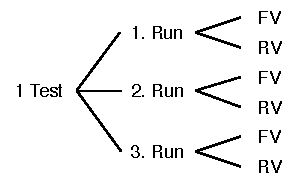
\includegraphics[]{runs}
\end{figure}

For one test, we have actually six times that the website gets loaded and tested.
For e.g. 500 URLs in the bulk test list, we have a total of $500 \times 6 = 3000$ page hits.


\paragraph{Configuration 1}

\begin{table}[h]
	\caption[Test Runs]{Configuration 1}
	\label{tab:tamodelleVergleich}
	\centering
	\begin{tabular}{ |c|c| } 
	\hline
	Configuration Setting & Option \\
	\hline
	Test Location & Test Location \\ 
	Browser & Chrome \\
	\hline
	Connection & LAN \\
	Number of Tests to Run & 3 \\
	Repeat View & First View and Repeat View \\
	Capture Video & True \\
	Keep Test Private & False \\
	Label & none \\
	\hline	  
	Advanced Tab & Nothing selected \\
	Chromium Tab & Nothing selected  \\
	Auth, Script, Block, SPOF, Custom Tabs & Nothing  \\
	Bulk Testing Tab & URL aramyesildeniz... 100 times \\
	\hline
	\end{tabular}
\end{table}

\paragraph{Configuration 2}

Emulate Mobile Browser




\subsection{Website Variations}

Positions:
1: Top of head element
2: just before closing head element
3: just before closing body element

\begin{center}
	\begin{longtable}{ |c|c|c|c|  }
	\hline
	Variant & Attribute & Position & Additional Scripts \\
	  \hline
	  \rowcolor{lightgrey}
	   Variant 1 & none & 1 & no \\
	  \rowcolor{lightgrey}
	  Variant 3 & async & 1 & no \\
	   & defer & 1 & no \\
	   
  	   & none & 2 & no \\
	   & async & 2 & no \\
  	   & defer & 2 & no \\

  	   & none & 3 & no \\
	   & async & 3 & no \\
  	   & defer & 3 & no \\
  	   
	  \rowcolor{lightgrey}
	   Variant 2 & none & 1 & yes \\
	   & async & 1 & yes \\
  	   & defer & 1 & yes \\

  	   & none & 2 & yes \\
	   & async & 2 & yes \\
  	   & defer & 2 & yes \\

  	   & none & 3 & yes \\
	   & async & 3 & yes \\
  	   & defer & 3 & yes \\
	  \hline
	\caption{Your caption here} % needs to go inside longtable environment
	\label{tab:myfirstlongtable}
	\end{longtable}
\end{center}

\paragraph{variant1.html}


\begin{center}
\begin{lstlisting}[caption={Variant 1},label=lst:soap,language=html,label={lst:soap}]
<!DOCTYPE html>
<html>
<head>
    <!-- Google Analytics -->
    <script>
            (function (i, s, o, g, r, a, m) {
            ...
    </script>
    <!-- End Google Analytics -->

    <meta charset="utf-8">
    <title>Median Website</title>
    <meta name="author" content="">
    <meta name="description" content="">
    <meta name="viewport" content="width=device-width, initial-scale=1">

    <!-- CSS / JS -->
    ...
</head>
<body>
...
</body>
</html>
\end{lstlisting}
\end{center}


\paragraph{variant2.html}

\paragraph{variant3.html}

\subsection{Plan}

The Google Analytics code is more or less fixed and there are no configurations.
It would be possible to change config of script, e.g. change sample rate, track other metrics etc.
But it is not possible to change default tracking behaviour (?)

How the script is included into the file should reflected withing Website Variations

% add Date as column? e.g. 2021-03-25
\begin{table}[h]
	\caption[Test Runs]{Test Runs \cite{DBLP:books/infix/Schwarz99}}
	\label{tab:tamodelleVergleich}
	\centering
	\begin{tabular}{ |c|c|c } 
	 \hline
	  WPT & Website & Date \\
	  \hline
	  C1 & V1 & 2021-04-01 \\ 
	  .. & .. & ..\\ 
	  \hline
	  \end{tabular}
\end{table}


\subsection{Tool support}

\begin{itemize}
\item python
\item Matplotlib
\end{itemize}
